% ----------------------
% THIS IS MY DEC1 REPORT
% ----------------------

\documentclass[titlepage,11pt,letterpaper]{article}

\usepackage{graphicx,epsfig,color}
\usepackage{subfigure}
\usepackage{setspace}
\usepackage{amsmath,amssymb}
\usepackage[hang,small,bf]{caption}
\usepackage[colorlinks]{hyperref}
\hypersetup{
	colorlinks=false,
	citebordercolor={0 1 0}
}
\setlength{\captionmargin}{10pt}
\setlength\parindent{0in}
\newcommand{\Matrix}[1]{\ensuremath \mathsf{#1}}
\newcommand{\Vector}[1]{\ensuremath \mathbf{#1}}
\newcommand{\Tensor}[1]{\ensuremath \vec{\vec{#1}}}
\newcommand{\Pfrac}[2]{\ensuremath \frac{\partial #1}{\partial #2}}
\newcommand{\Rfrac}[2]{\ensuremath \frac{\mbox{d} #1}{\mbox{d} #2}}
\newcommand{\Dvolume}{\ensuremath {d\Omega}}
\newcommand{\Dsurface}{\ensuremath dS}
\newcommand{\Intvolume}[1]{\ensuremath \int_\Omega {#1}\Dvolume}
\newcommand{\Intsurface}[1]{\ensuremath \int_{\Dvolume} {#1}\Dsurface}
\newcommand{\Intsurfacedot}[1]{\ensuremath \int_{\Dvolume} {#1}\cdot\Vector{\Dsurface}}
\newcommand{\Div}[1]{\ensuremath \Vector{\nabla}\cdot#1}
\newcommand{\Grad}[1]{\ensuremath \Vector{\nabla #1}}
\newcommand{\Sumedges}{\ensuremath \sum_{ik}^{\text{edges}}}
\newcommand{\nutilde}{\ensuremath \tilde{\nu}}
\newcommand{\Dx}{\ensuremath \Delta x}
\newcommand{\Dy}{\ensuremath \Delta y}
\newcommand{\Ds}{\ensuremath \Delta s}
\newcommand{\Dl}{\ensuremath \Delta l}
\newcommand{\Dt}{\ensuremath \Delta t}
\newcommand{\Tilda}[1]{\ensuremath \mbox{\~{#1}}}
\newcommand{\pseudo}{\ensuremath \textrm{\textdied}}
%\newcommand{\Fi}{\ensuremath{\mathbf{F}_{\boldsymbol{\iota}}} }
\newcommand{\Fi}{\ensuremath{\mathbf{F}} }
\newcommand{\Fv}{\ensuremath{\mathbf{F}_{\boldsymbol{\nu}}}}
%\newcommand{\Gi}{\ensuremath{\mathbf{G}_{\boldsymbol{\iota}}} }
\newcommand{\Gi}{\ensuremath{\mathbf{G}} }
\newcommand{\Gv}{\ensuremath{\mathbf{G}_{\boldsymbol{\nu}}} }
%\newcommand{\Hi}{\ensuremath{\mathbf{H}_{\boldsymbol{\iota}}} }
\newcommand{\Hi}{\ensuremath{\mathbf{H}} }
\newcommand{\Hv}{\ensuremath{\mathbf{H}_{\boldsymbol{\nu}}} }
\newcommand{\etal}{\textit{et al}}

\newcommand{\pd}[2]{\frac{\partial#1}{\partial#2}}
% Page Margins
\voffset=-1.0in
\topmargin=0.75in
\headheight=0.0in
\headsep=0.0in
\hoffset=-1.0in
\oddsidemargin=0.7in
\evensidemargin=0.7in
\bibliographystyle{unsrt}
\parindent      0.2000in

\textwidth=7.0in
\textheight=9.25in

% Line Spacing
\renewcommand{\baselinestretch}{1.33}

% Alter some LaTeX defaults for better treatment of figures:
% See p.105 of "TeX Unbound" for suggested values.
    % See pp. 199-200 of Lamport's "LaTeX" book for details.
    %   General parameters, for ALL pages:
    \renewcommand{\topfraction}{0.9}	% max fraction of floats at top
    \renewcommand{\bottomfraction}{0.8}	% max fraction of floats at bottom
    %   Parameters for TEXT pages (not float pages):
   \setcounter{topnumber}{2}
    \setcounter{bottomnumber}{2}
    \setcounter{totalnumber}{4}     % 2 may work better
    \setcounter{dbltopnumber}{2}    % for 2-column pages
    \renewcommand{\dbltopfraction}{0.9}	% fit big float above 2-col. text
    \renewcommand{\textfraction}{0.07}	% allow minimal text w. figs
    %   Parameters for FLOAT pages (not text pages):
    \renewcommand{\floatpagefraction}{0.7}	% require fuller float pages
	% N.B.: floatpagefraction MUST be less than topfraction !!
    \renewcommand{\dblfloatpagefraction}{0.7}	% require fuller float pages

    % remember to use [htp] or [htpb] for placement

%\newcommand*{\drop}{\vspace*{0.2\textheight}}
\newenvironment{absolutelynopagebreak}
  {\par\nobreak\vfil\penalty0\vfilneg
   \vtop\bgroup}
  {\par\xdef\tpd{\the\prevdepth}\egroup
   \prevdepth=\tpd}
   
   
\usepackage{chngcntr}
\counterwithin*{equation}{section}
\counterwithin*{equation}{subsection}   
\numberwithin{equation}{subsection}


\begin{document}


\newcommand*{\titleRR}
{\begingroup
  \centering
  \vfill
  \begin{figure}
    \vspace{1.5cm}
    \begin{center}
      
\includegraphics[width=0.17\textheight]{./figs/utias_logo_blue.jpg}
    \end{center}
    \vspace{1.5cm}
  \end{figure}
  {\LARGE \textbf{Development of h-p adjoint-based error estimation for LES of reactive flows}}\\
  \vspace*{2.0cm}
  {\large Christopher Ngigi}\\
  \vspace*{1.cm}
  {\normalsize\itshape University of
    Toronto Institute for Aerospace Studies}\\
  {\normalsize\itshape 4925
    Dufferin Street, Toronto, Ontario, M3H 5T6, Canada}\\
  \vspace*{2.cm}
  {Doctoral Examination Committee I Report} \\
  \vspace*{1.cm}
  {April 2015}
  \vfill\null
\endgroup}

\thispagestyle{empty}\titleRR
\clearpage
\setcounter{page}{1}

%\maketitle
%\tableofcontents
%\newpage

%%%%%%%%%%%%%%%%%%%%%%%%%%%%%%%%%%%%%%%%%%%%%%%%%%%%%%%%%%%%%%%%%%%%%%%%%%%%%%%%%%%%%%%%%%%%
%-------------------------------------------------------------------------------------------
% Introduction and Motivation
%-------------------------------------------------------------------------------------------
%%%%%%%%%%%%%%%%%%%%%%%%%%%%%%%%%%%%%%%%%%%%%%%%%%%%%%%%%%%%%%%%%%%%%%%%%%%%%%%%%%%%%%%%%%%%
\newpage
\section{Introduction and motivation}

The development of computational fluid dynamics (CFD) over the past 30-40 years has been carried out with a goal of helping to reduce the time and cost of prototype design for a wide range of engineering systems. Practical reactive flows almost always involve turbulence, and CFD methods have been developed to help capture such complex phenomena to varying extents of accuracy. The corresponding physical experiments can, in many cases, take a long time and be very expensive to conduct. Three main numerical approaches exist for the treatment of turbulent flows. Reynolds averaged Navier Stokes (RANS) uses full modeling of the turbulent scales; Large eddy simulations (LES) model sub-filter scales (SFS) while resolving larger scales; and Direct numerical simulations (DNS) resolve all the turbulent scales. Supercomputers have been used within academic and research lab collaborations for the DNS of canonical cases such as turbulence in a box as considered by Kaneda and Ishihara~\cite{kaneda:2006}, but such calculations are very expensive and limited to simple cases with low Reynolds numbers. More complicated analyses such as those involving combustion simulations use LES to achieve an overall good prediction of results at an accuracy greater than RANS, but at a cost lower than DNS.\par 

To improve the accuracy of LES, we need to reduce and control the error within the simulation. Key sources of error in CFD include numerical and modeling errors. Modeling errors in LES can be significantly reduced by using explicit discrete commutative filters. Numerical errors can be reduced by applying mesh refinement ($h$ refinement) or by increasing the polynomial discretization of the numerical scheme ($p$ refinement). High order discretizations, generally classified as those having order $p>2$, have less numerical dissipation and require fewer mesh points to achieve solution accuracy (as compared to a $2^{nd}$ order method, for example). To minimize the computational costs, refinement would be \textit{localized} i.e.\ applied specifically to regions of high error. Ways to quantify the error include the gradient (physics)-based approach, but this technique does not guarantee error reduction for continual levels of mesh refinement($h$ refinement).  (More on gradient-based methods will be discussed in Section \ref{section:Adjoint}). A more effective approach to derive a set of defined error estimates is the adjoint-based method, where localized numerical errors are obtained at a potentially lower cost. This work proposes the combination of $h$ refinement with $p$ refinement within an adjoint-based error estimation framework. That is, the additional use of high-order discretization schemes  to further improve accuracy of the CFD results, while lowering the cost to attain them. This combination, expressed as an adjoint-based $\mathcal{O}(h^p)$ error estimation technique, will allow for better assessment and control of error.\par 

%%%%%%%%%%%%%%%%%%%%%%%%%%%%%%%%%%%%%%%%%%%%%%%%%%%%%%%%%%%%%%%%%%%%%%%%%%%%%%%%%%%%%%%%%%%%
% Scope of Research
%%%%%%%%%%%%%%%%%%%%%%%%%%%%%%%%%%%%%%%%%%%%%%%%%%%%%%%%%%%%%%%%%%%%%%%%%%%%%%%%%%%%%%%%%%%
\section{Scope of research}

\begin{itemize}

\item The goal is Reducing numerical error using high order CENO and adjoint based error estimation, $\mathcal{O}(h^p)$ $\rightarrow$ $h$ and $p$ adaptation

\item This work proposes a two-pronged technique to reduce the numerical error within the discretized governing equations, as well as in the computational domain (mesh).  Implementation of high order finite volume method (FVM) as well as adjoint-based error estimation is believed to be a significant step to achieve this. The adjoint technique can be used for $\mathcal{O}(h^p)$ refinement: evaluating error estimates and then locally switching between h and p refinement, based on the computational cost savings.

\item The CFFC code already has most of the needed formulations required for this work. 
\begin{itemize}
\item Combustion modeling:
  \begin{itemize}
   \item PCM-FPI: This model allows detailed chemical kinetics via tabulation of precomputed laminar premixed flames, and has already been implemented within the CFFC code by H. Perez (2011) ~\cite{hperez:2011a}
   \end{itemize}  

\item Favre-filtered Navier Stokes governing equations: The FANS formulation has already been implemented within the group CFFC code.
      
\item Large Eddy Simulation:
  \begin{itemize}
   \item Explicit filtering work done by Deconinck, ~\cite{Deconinck:2008}
   \item Sub-filter scale (SFS) modeling work done by H. Perez ~\cite{hperez:2011a}
  \end{itemize}

\item High-order finite volume methods: CENO technique - benefits of higher accuracy on a coarse mesh was implemented by Ivan and Groth ~\cite{ivan:2007, ivan:2013b}

\item AMR
   \begin{itemize}
   \item Block-based AMR: speed and parallelization [Groth et al 1999]
   \item Anisotropic AMR reduces cell count (computational cost): 2-D initial work by Zhang and Groth \cite{zhang:2011b}, and extended to 3-D by Williamschen and Groth \cite{Williamschen:2013}
   \item Freret and Groth, \cite{Freret:2015} extended the work of Williamschen to include a non-uniform block formulation. This increases code accuracy while saving computational resources.
   \end{itemize}
   
\item Solution method: Northrup and Groth~\cite{Northrup:2013, northrup:2013a} implemented an implicit GMRES solver that improves the robustness and capability of the CFFC code by relieving it from the Courant-Friedric-Levy (CFL) condition constraints.  

\end{itemize}

\item Workflow: 
\begin{itemize}
	\item Creating a framework for the adjoint based error estimation method. The approach to be used will be to first formulate the adjoint solver within the group CFFC Code. 
	\item Once the adjoint is formulated, it will be validated on already known inviscid (Euler) laminar steady solutions, and then implemented for unsteady cases. Complexity will be introduced by adding viscosity and then a temporal variation. 
	\item The next step will be to advance the work done by Deconinck on explicit filters and implement them \cite{Deconinck:2008} to the high-order FVM scheme. 
\end{itemize}

\item The implementation of the adjoint based error estimation would allow for significant reductions in numerical error, and these will be accounted for in the duration of this research.
\end{itemize}




%%%%%%%%%%%%%%%%%%%%%%%%%%%%%%%%%%%%%%%%%%%%%%%%%%%%%%%%%%%%%%%%%%%%%%%%%%%%%%%%%%%%%%%%%%%%
%-------------------------------------------------------------------------------------------
% CFD Techniques to Model Combustion
%-------------------------------------------------------------------------------------------
%%%%%%%%%%%%%%%%%%%%%%%%%%%%%%%%%%%%%%%%%%%%%%%%%%%%%%%%%%%%%%%%%%%%%%%%%%%%%%%%%%%%%%%%%%%%
\section{Proposed Adaptive Mesh Refinement Strategy}

The planned approach to perform the Adjoint-based Error Estimation (covered in Section \ref{section:Adjoint}) will utilize the following techniques

\subsection{Large eddy simulation (LES)}
The level of fidelity of LES lies between the fully resolved Direct Numerical Simulation (DNS) and the fully modelled Reynolds-Averaged Navier Stokes (RANS) methods. LES applies a filter size ($\bar{\Delta}$) to the turbulence scales, resolving the larger ones, and modelling those smaller than the filter size. Flow variables need to be decomposed into filtered(resolved) and residual (modelled or Sub-Filter Scale (SFS)) components via a spatial filtering procedure. Consequently, the Navier Stokes Equations (Section \ref{section:Navier}) need to be Favre-filtered (Section \ref{section:Favre}) before being used in LES. Two main techniques for Filtering are used: implicit and explicit filtering.\par  

In implicit filtering, the filter width is not explicitly defined and is inherently related to grid resolution. The main disadvantage is that it is difficult to compare results of adapted/refined meshes. Hence there is need for explicit filtering, whereby Define $\bar{\Delta} $ is fixed for the entire mesh, and convergence tests are more consistent. \cite{HPerez:2011, Deconinck:2008}


\subsubsection{Aliasing errors} \label{section:aliasing_errors}
As a result of Favre filtering on the governing equations, (see section \ref{section:Favre}) a non-linear correlation will result:\par
\begin{equation}
 \frac{\partial \;\;}{\partial x_\mathrm{j}} (\overline{\rho u_\mathrm{i} u_\mathrm{j}}) \: ,
 \end{equation}
This creates a closure problem. To solve this, the product of the closed filtered velocities is evaluated and the remaining term is modeled, essentially transfering the closure problem to the right-hand side of the filtered Navier-Stokes equation:
\begin{equation}
\overline{\rho u_\mathrm{i} u_\mathrm{j}} = \bar{\rho} \tilde{u}_\mathrm{i} \tilde{u}_\mathrm{j} 
+\underbrace{ (\overline{\rho u_\mathrm{i} u_\mathrm{j}} - \bar{\rho} \tilde{u}_\mathrm{i} \tilde{u}_\mathrm{j} ) }_{\sigma_\mathrm{ij}} \: ,
\end{equation}
where $\sigma_\mathrm{ij}$ is the SFS stress tensor. This decomposition leads to the non-linear product $\tilde{u}_\mathrm{i} \tilde{u}_\mathrm{j}$ generating frequencies that are beyond the characteristic frequency that defines $\tilde{u}_\mathrm{i}$~ and act as fictitious stresses \cite{Lund:03}.
The resulting errors are difficult to eliminate and control if implicit filtering is used. Explicit filtering allows control of these. Please refer to the work of H. Perez \cite{HPerez:2011} and Deconinck~\cite{Deconinck:2008} for additional details.\par

\subsubsection{Commutation errors} \label{section:commutation_errors}
For most inhomogeneous turbulent flows, the smallest eddy sizes that can be resolved differ in various regions of the flow. Usually, flow close to solid walls  produces smaller eddies due to damping effects. This implies that the mesh should be refined to resolve these scales in the near-wall region. To ensure the structure of filtered equations remains unchanged before and after filtering, the filtering operation should commute with the differential operation, and this is described by H. Perez \cite{HPerez:2011} as follows: 
\begin{equation} 
\overline{\frac{\mathrm{d} \phi}{\mathrm{d} x} } = \frac{\mathrm{d} \bar{\phi}}{dx} \: .
\end{equation}
In general, filters do not commute when variable filter width is used. To be acceptable, the errors associated with the commutation properties of the filter should be of the same order as the truncation errors associated with the numerical scheme, i.e.,
 \begin{equation} \label{eq:commutation_error}
\left[ \frac{\mathrm{d} \phi}{\mathrm{d} x}   \right]  \equiv \left| \overline{\frac{\mathrm{d} \phi}{\mathrm{d} x} } - \frac{\mathrm{d} \bar{\phi}}{\mathrm{d}x}\right| = \mathcal{O}(\Delta^n) \: ,
\end{equation}
 where $n$ is the order of the filter, which should be at least equal to the order of accuracy of the spatial discretization scheme. Thus for a $p^{th}$ order numerical scheme, $n = p$.


\subsubsection{Sub-filter scale (SFS) modelling}
The SFS terms (see section ~\ref{section:Favre}) need to be modeled in LES, since they have a pronounced effect on the resolved scales. The energy cascade, first described by Richardson in 1922, explains how the Turbulent Kinetic Energy is mainly contained in the larger scales, and dissipated by the smallest scales via viscosity.\cite{Pope:2005}.\par
A number of approaches have been used to model the SFS terms. One of the first was by Smagorinsky \cite{Smagorinsky:1963} which models SFS stress tensors and the Reynolds' stress tensor. This approach also defines a SFS eddy viscosity which is in turn used to relate SFS stresses to the filtered strain rates, based on the assumption that the SFS stress tensor behaves similar to the viscous stress tensor, itself proportional to the Strain rate tensor. The model goes ahead to express the SFS eddy viscosity as proportional to the magnitude of the filtered strain rate tensor. The constant of proportionality is termed the Smagorinsky Coefficient. In the case where the Smagorinsky coefficient is valid only for an optimized flow regime, we obtain the dynamic Smagorinsky model. This will likely be the model of choice for this research.

\subsection{The finite volume method}
Godunov-type Finite Volume Methods (FVM) will typically apply a cell-centered spatial discretization. This results in the splitting of the solution domain into control volumes ~\cite{Toro:1997}. The integral form of the governing equations is applied. The Navier Stokes and Favre-Averaged Navier Stokes are described in the Appendix, see Section ~\ref{section:Navier} and ~\ref{section:Favre}.\par 
The Favre-filtered form of the conservation equations for mass, momentum, total energy, and species mass fractions, along with the equation of state are used here in the LES of turbulent reactive flows and can be re-expressed in the following general weak conservation form using matrix-vector notation ~\cite{Neto:2014}
%%
\begin{equation}
\label{eq:weak.form}
\frac{\partial \overline{\Vector{U}}}{\partial t} 
+ \vec{\nabla} \cdot \vec{\mathcal{F}} =
\frac{\partial \overline{\Vector{U}}}{\partial t} + 
\vec{\nabla} \cdot \vec{\mathcal{F}}^{\mathrm{I}} \left( \overline{\Vector{U}} \right) - 
\vec{\nabla} \cdot \vec{\mathcal{F}}^{\mathrm{V}} 
\left( \overline{\Vector{U}}, \vec{\nabla} \overline{\Vector{U}} \right) = 
\overline{\Vector{S}}
\end{equation}
%%
where $\overline{\Vector{U}}$ is the vector of conserved solution variables and $\vec{\mathcal{F}}$ is the solution flux dyad.  The flux dyad can further be decomposed into two components and written as $\vec{\mathcal{F}} =  \vec{\mathcal{F}}^{\mathrm I} - \vec{\mathcal{F}}^{\mathrm{V}}$ where $\vec{\mathcal{F}}^{\mathrm I} = \vec{\mathcal{F}}^{\mathrm I}(\overline{\Vector{U}})$ which contains the hyperbolic or inviscid components of the solution fluxes, and  $\vec{\mathcal{F}}^{\mathrm{V}} =  \vec{\mathcal{F}}^{\mathrm{V}}(\overline{\Vector{U}}, \vec{\nabla} \overline{\Vector{U}})$ which contains the elliptic or viscous components of the fluxes.

Inviscid fluxes (the hyperbilic part) within each cell (control volume) are resolved via a solution to a Riemann Problem, given the different left and right states for each cell. The goal is to obtain the final cell-centered, cell-average value. Typically, approximate Riemann solvers are used to this end.

For the purpose of CFD, these governing equations in PDE form need to be discretized. The integral form of Eq.~(\ref{eq:weak.form}) is applied to a hexahedral reference cell $(i,j,k)$ and an $N_G$-point Gaussian quadrature numerical integration procedure is used to evaluate the solution flux along each of the $N_f$ faces of the cell, to obtain:

\begin{equation}
\label{eqn:semi_discrete}
 \frac{\mathrm{d}\overline{\Vector U}_{ijk}}{\mathrm{d}t} =
 - \frac{1}{{V}_{ijk}} \sum_{l=1}^{N_f} 
 \sum_{m=1}^{N_{GF}} \left( \omega_m \left(\vec{\mathcal{F}^{\mathrm{I}}} - 
 \vec{\mathcal{F}^{\mathrm{V}}} \right)\cdot \hat{n} {A} \right)_{ijk,l,m}
 + \sum_{n=1}^{N_{GV}} \left( \omega_n {\Vector S} \right)_{i,j,k,n}
 = \overline{\Vector{R}}_{ijk} \left( \overline{\Vector{U}} \right),
\end{equation}
where $\omega_m$ are the face quadrature weighting coefficients, $\omega_n$ are the volumetric quadrature weighting coefficients, $A_l$ denotes the surface area of face $l$, and $\overline{\Vector{R}}_{ijk}$ is the residual operator. After the evaluation of $\overline{\Vector{R}}$, one can advance the solution in time, and therefore iteratively solve the time dependent problem that is described by the equations. Quadrature rules are used to determine the Flux evaluation points on the surface, $N_{GF}$ and those for the volume, $N_{GV}$. The remaining procedure is:
\begin{itemize}
\setlength\itemsep{0.1em}
 \item Apply Solution Reconstruction (see ~\ref{section:CENO});
 \item Evaluate the Inviscid and Viscous Fluxes and apply the weights to respective Gauss-Legendre points;
 \item Evaluate the Source Vector, which adds effects of turbulence and chemistry in reacting flows;
 \item Apply an appropriate time-marching scheme, such as a fourth-order Runge-Kutta (RK4) suitable for High-Order methods.
\end{itemize}
High-Order generally refers to $k>2$. These kind of methods generally have less numerical dissipation, require fewer mesh points to achieve solution accuracy, (as compared to a $2^{nd}$ Order method, for example)

\subsubsection{The centrally essentially non-oscillatory (CENO) scheme}
\label{section:CENO}
In solution reconstruction, given cell average values, a Taylor series expansion polynomial is defined to represent the variation of the solution within the particular cell and the average solution of its neighbors. \par
The High-Order CENO reconstruction scheme of Ivan and Groth [~\cite{ivan:2007}, \cite{ivan:2013b}] uses a \textit{k}-exact least-squares reconstruction technique, essentially a $k^{th}$ order Taylor series expansion of solution variable $U$ about the cell center. This technique is applied to a monotonicity-preserving limited linear scheme. For Favre-Averaged Navier Stokes (FANS), \textit{k} corresponds to the spatial accuracy of the scheme. A smoothness indicator is used to switch between reconstruction procedures.\par
Some of the advantages of CENO are ~\cite{Groth:2013}:
\begin{itemize}
\setlength\itemsep{0.1em}
\item It provides accuracy of other Essentially Non-Oscillatory (ENO) schemes and maintains monotonicity near discontinuities;
\item Identifies regions where under-resolution and non-smooth data occurs, and this could prove useful for mesh adaptation techniques.
\end{itemize}


\subsection{Block-Based Adaptive Mesh Refinement (AMR)}
Having discretized the governing equations, the geometry similarly needs to be discretized into unique cells, in a process called meshing. For increase in accuracy, a finer mesh resolution (smaller grid size) will be required. \par

Adaptive Mesh Refinement (AMR) takes its name from the variational increase in localized grid resolution to allow for improved accuracy at without carrying out the same at a ubiquitous scale. Global refinement is often cheaper to perform, whereas localized (Adaptive) is not; however, the computational cost for refining many more cells and storing this information makes it more expensive, in spite of the fact that a well designed approach selection will need to be programmed to perform an adaptive refinement.\par
Block-based AMR groups cells into blocks, making it an optimal configuration for parallel systems, where each processor could have a certain number of Blocks, and protocols such as the Message Passing Interface (MPI) could be used for Block-Block inter-communication. Communication between Blocks occurs via Ghost cells, and in case neighboring blocks have a difference in mesh resolution, then Mutligrid-type restriction and prolongation is used.\par

Groth \etal ~\cite{Groth:1999} developed some of the initial work with Block-Based AMR for Computational Magnetohydrodynamics, and was extended to enable parallel implementation for a variety of complex flows. Northrup and Groth ~\cite{Northrup:2005b} implemented a fully-implicit, parallel Newton-Krylov method, and applies Schwarz preconditioning to take advantage of the Block structure of the computational grid.
Within Block-based AMR, the cell-connectivity is stored in a tree structure, which will typically be an octree in a 3D domain. Block-Based AMR is more optimized than a refinement performed on a cell-by-cell basis, as the information storage process for the latter is computationally expensive: The tree approach is much simpler, faster and cheaper. Blocks flagged for increased  resolution can be refined using two approaches: \par

%parallel here


\begin{enumerate}

\item \textbf{Isotropic AMR}:\\
Isotropic AMR  occurs by uniformly splitting the Parent cell into 8 children (in a 3D domain) or into 4 children (in a 2D domain). This considers that the physics is occurring without a preference for a given direction, and usually results in a larger-than-desired cell count.
\begin{figure}[t!]
  \centering
   \subfigure[Mesh for Isop]
   {\label{fig:Poisson 2D}	   
   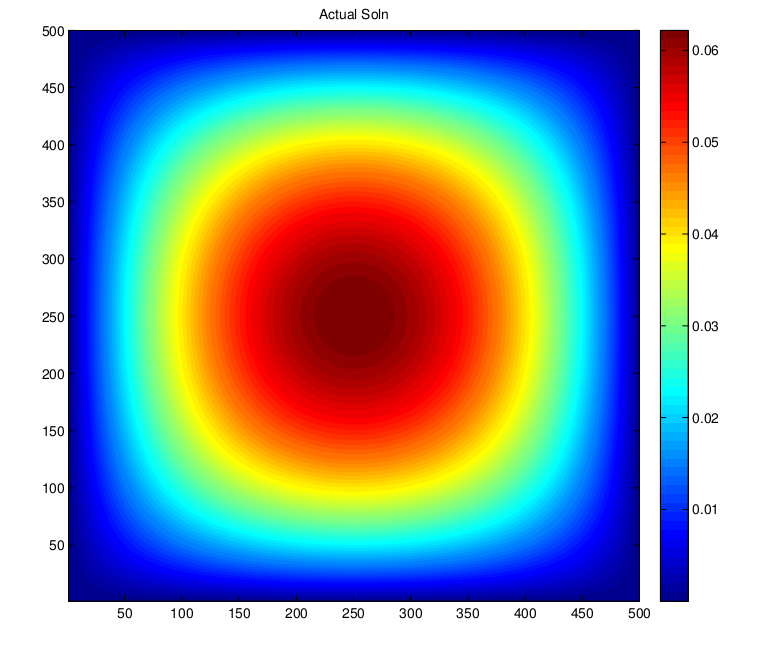
\includegraphics[height=0.4\textwidth, trim=0.2cm 0.2cm 0.2cm .2cm,clip=true]{figs/Poisson2D.png}}%
     %% 
	\:
	\subfigure[3D case on N$^3$ $= 100^3$]
   {\label{fig:Poisson 3D}	   
   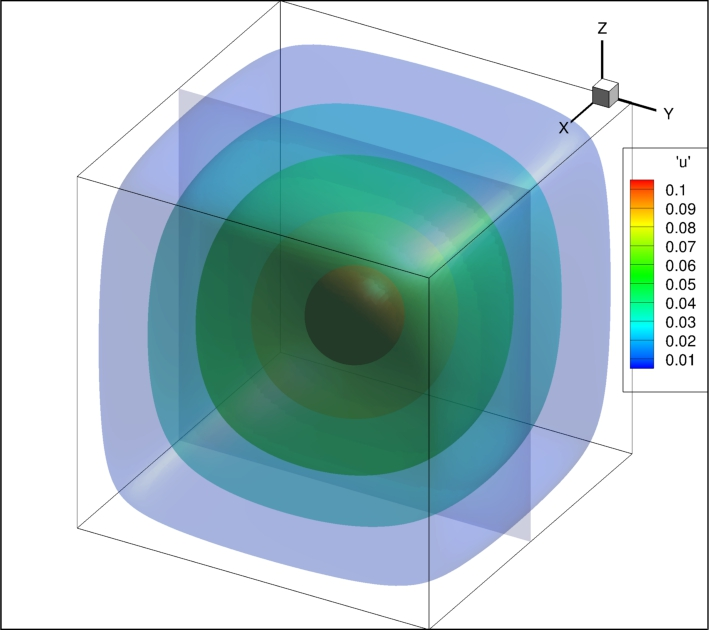
\includegraphics[height=0.4\textwidth, trim=0.2cm 0.2cm 0.2cm .2cm,clip=true]{figs/Poisson3D.jpeg}}%
     %%\caption{Solution Contours for the 3D solution of the Poisson Problem}  
     
    \caption{Solution Contours for solution of the Poisson Problem}  
\end{figure}

\item \textbf{Anisotropic AMR}: \\
For flows having a directional bias, e.g. in the simulation of a jet exiting a nozzle, the dominant direction will be along the axis of symmetry of the nozzle. Therefore, a priori, we can tell that the mesh cells would ideally need to be stretched along this same axis. Whenever we have this kind of bias on the cell geometry, we have anisotropy. Mesh refinement occurs in a slightly different manner, as now we switch to a binary tree system, which stores refinement history and cell connectivity. Two, four, or eight refined
blocks can be created, resulting in five distinct possible refinements for a single block to better adapt to evolving flow features. Studies by Zhang ~\cite{Zhang:2011b}, and Zhang and Groth ~\cite{Zhang:2011a} indicate that Anisotropic AMR for given simulations result in lower cell counts, although the refinement procedure is more difficult than that of the Isotropic AMR.\par
Freret and Groth \cite{Freret:2015} have completed a new formulation for a Non-uniform block-based approach that targets the the ghost cells. In this method, a block will copy over the mesh resolution and solution information of its neighboring block to its own ghost cells, and this eliminates the interpolation error within a Uniform block-based scheme that would otherwise have resulted in necessary solution restriction and prolongation (if the mesh discretization levels were different). Further, this saves the computational cost of flux correction cycles, done via message passing between the blocks, as described by Zhang to be a temporary remedy to ghost-cell evaluation.\cite{Zhang:2011a}

\end{enumerate}


\subsection{Combustion modeling via the presumed conditional moment and flame propagation for intrinsic low-dimensional manifold (PCM-FPI) model}

When performing LES of turbulent reactive flows, there is need to predict the chemical reaction rates. Implementation of the PCM-FPI model in LES within the CFD Group was carried out by Hern{\'a}ndez-P{\'e}rez ~\cite{HPerez:2011} and Shahbazian \etal ~\cite{Shahbazian:2011}.\par

The FPI model was proposed to build databases based on detailed simulations of simple flames. The basis of tabulations is the steady-state one-dimensional laminar flame, which are solved using CANTERA software. These flame quanitities are stored in a table that is then read by the CFFC program. The main objective of the FPI tabulation technique is to reduce the cost of performing reactive
flow computations with large detailed chemical kinetic mechanisms, but still retain the accuracy of detailed results, by building databases of relevant quantities based on detailed simulations of simple flames. ~\cite{HPerez:2011} \par

The PCM technique uses a statistical approach and utilizes Probability Density Functions (PDFs). The approach presumes a PDF-like distribution of a subfilter-scale fluctuating quantity. The PDF subfilter is incorporated into the Favre-filtered reaction rates for species.\par

Combining PCM with FPI allows an approach to model complex chemistry from tabulated data, is a very general model that can be used for premixed, non-premixed and partially-premixed flames. e.g. In the event that turbulent premixed combustion is the focus of the analysis, look up tables of filtered terms are built up from laminar premixed flamelet data.\par


%%%%%%%%%%%%%%%%%%%%%%%%%%%%%%%%%%%%%%%%%%%%%%%%%%%%%%%%%%%%%%%%%%%%%%%%%%%%%%%%%%%%%%%%%%%%
%-------------------------------------------------------------------------------------------
% Adjoint Method for Error Estimation
%-------------------------------------------------------------------------------------------
%%%%%%%%%%%%%%%%%%%%%%%%%%%%%%%%%%%%%%%%%%%%%%%%%%%%%%%%%%%%%%%%%%%%%%%%%%%%%%%%%%%%%%%%%%%%
\section{Adjoint-based method for error estimation}
\label{section:Adjoint}
\subsection{Introduction}

In Gradient-based Mesh adaptation techniques, emphasis is placed on the change of values of the Solution variables across cells, and any high rates of change require a mesh refinement suitable enough to capture a smoother transition, e.g. across a shock wave that forms on the upper surface of an airfoil in transonic regime. In this scenario, a quantity such as density or pressure could be monitored.\par

To make error estimation more relevant to engineering applications it is useful to assess the error made in predicting an integral quantity which represents an engineering output. This output is called the functional. For example,the output can be the average pressure on a wall. The adjoint technique is a sensitivity analysis, that measures the rates of change of a design functional to a given change in the input. \par

Extensive research has been performed by Giles and Pierce ~\cite{Giles:2000}, Becker and Rannacher~\cite{Becker:2001}, Venditti and Darmofal~\cite{Venditti:2000, Venditti:2002} and a review carried out by Fidkowski and Darmofal ~\cite{Fidkowski:2011}.

The adjoint has two main formulations: the continuous and the discrete.\par

In the \textit{continuous} approach, an objective function is formed to enforce the flow conditions (i.e. primal nonlinear PDEs). Next, linear perturbations to the primal flow variables are considered, while enforcing the objective function to remain constant with respect to the perturbations. As a result, analytical adjoint equations are obtained, and relevant boundary conditions applied. The formulation is then discretized directly. \par

For the \textit{discrete} formulation, the nonlinear discrete residual equations from the primal problem are the starting point, and, similar to the continual approach, linear perturbations are applied. If the system is adjoint consistent, i.e. discrete adjoint = continuous adjoint, then there is no need for boundary condition specification. These get automatically incorporated via the primal residual. Finally, a linear system of equations is established with the only necessary evaluation being the linear sensitivities of the functional and the Jacobian matrix associated with the primal residual. \par

Adjoint-based Error Estimation focuses on the \textit{sensitivities}, whereby some output of interest (henceforth termed as a \textit{functional}), e.g. Lift on an airfoil, is sensitive to the mesh refinement levels upstream of the airfoil along the chord line. The Adjoint approach is a more efficient, albeit expensive, criteria for mesh refinement: only one calculation for the sensitivity needs to be calculated, whereas for gradient based approaches, each quantity will require a unique calculation.\par

The adjoint-based method applies a \textit{posteriori} technique, in that an initial solution, known as the \textit{Primal solution}, needs to first be evaluated - no refinement criteria can be carried out until the primal solution is established. Once this is met, error estimates can be evaluated from the adjoint, and this could be used as a mesh refinement criteria. \par

Other key research on adjoints applied to aerodynamic flows was performed by Giles and Pierce ~\cite{Giles:2000}, Becker and Rannacher ~\cite{Becker:2001} and Venditti and Darmofal ~\cite{Venditti:2003}, with a key summary done by Fidkowski and Darmofal \cite{Fidkowski:2011}.


\subsection{Derivation}
If \textbf{R} is the set of all residuals for all cells in the domain, then the systems of equations can be written as:
\begin{equation}
\textbf{R}(\textbf{U}) = 0
\end{equation}
Considering a scalar output of interest \cite{Fidkowski:2013}, say, $J$, we can define it such that:
\begin{equation}
J = J(U)
\end{equation}
where U is a vector containing the solution variable. We define a discrete Adjoint, $\Psi \in \mathbb{R}^N$ as a vector of sensitivities of the output to the $N$ residuals. Each entry of the adjoint essentially tells us the effect that a perturbation in the corresponding entry within the residual vector would have on output $J$. Consider the case fo a residual perturbation due to a change to the input parameter, $\mu$, and $\mu \in \mathbb{R}^{N_p}$. A local sensitivity analysis can be applied as follows:\par
\begin{equation} \label{eqn:chain}
\underbrace{\mu}_{\text{inputs} ~\in~\mathbb{R}^{N_\mu}} ~\to~ \underbrace{\textbf{R}(\textbf{U},\textbf{$\mu$}) = 0}_{\text{\textit{N} equations}} ~ \to ~ \underbrace{\textbf{U}}_{\text{state} ~\in~ \mathbb{R}^N} ~\to~ \underbrace{\text{\textit{J}(\textbf{U})}}_\text{output(scalar)} 
\end{equation}

To monitor the change of $J$ with $\mu$,
\begin{equation}
\frac{dJ}{d\mu} ~\in~ \mathbb{R}^{1~\times~N_{\mu}} = N_\mu ~ \text{sensitivities}
\end{equation}

recalling $\mu \in \mathbb{R}^{N_p}$. If $J$ depended directly on $\mu$ then we would have had $\frac{dJ}{d\mu}$, but in the scenario we consider the case that $J = J(U)$ alone. To evaluate the $N_\mu$ sensitivities we could use: \textit{finite differencing} where the inputs are  perturbed one at a time;  \textit{forward linearization} where the sequence of operations in Equation ~\eqref{eqn:chain} are linearized; and, lastly, the \textit{adjoint approach} which requires an inexpensive residual perturbation calculation, followed by an adjoint weighting to compute the effect on the output:\par
\begin{equation}
\frac{dJ}{d\mu} = \Psi^T ~\frac{\partial R}{\partial \mu}
\end{equation}
One of the key ideas behind the adjoint approach is that the forward problem need be solved only once to evaluate a sensitivity. Given a particular input, $\mu$, we could solve the system to find \textbf{U} such that \textbf{R(U,$\mu$} $ = 0$. Once we perturb $\mu ~\to~ \mu + \delta \mu$, to find the effect on $J$, we would otherwise need to re-solve the discretized system, which would be an expensive step. The Adjoint, on the other hand, precomputes the eddect of \textbf{R} on $J$. The resulting $N$ sensitiviteis are stored in vector $\Psi$.\par

Consider the chain of events in computing sensitivities (i.e. the effects of a small perturbance of the input, $\delta \mu$) via a direct approach:
\begin{enumerate}
\item Input:  $\mu ~\to~ \mu + \delta \mu$
\item Residual: \textbf{R(U, $\mu ~+~ \delta \mu$)} $=$ $\delta$\textbf{R} $\neq 0$ ~$\to$~ \textbf{R(U, $\mu$)} $+$ $\frac{\partial \text{\textbf{R}}}{\partial \mu}$ $\bigg|_{\textbf{U, $\mu$}}$ $\delta \mu = \delta$\textbf{R}
\item State: \textbf{R(U $+ \delta$U, $ \mu + \delta\mu$)} $= ~0$ ~$\to$~ \textbf{R(U, $\mu$)} $+$ $\frac{\partial \text{\textbf{R}}}{\partial \mu}$ $\bigg|_{\textbf{U, $\mu$}}$ $\delta \mu$ $ + \frac{\partial \text{\textbf{R}}}{\partial \text{\textbf{U}}}$     $\bigg|_{\textbf{U, $\mu$}} \delta$U  $ = 0$
\item Output: $J(\textbf{U} + \delta \textbf{U}) = J(\textbf{U}) + \delta J ~\to~ \delta J = \frac{\partial J}{\partial \textbf{U}} \delta U $
\end{enumerate}

Subtracting step 2 from 3:
\begin{equation}
\begin{split}
\frac{\partial \textbf{R}} {\partial \textbf{U}} \bigg|_{\textbf{U, $\mu$}} \delta U &= - \delta R \\
\delta \textbf{U} &= - \left[\frac{\partial \textbf{R}}{\partial \textbf{U}} \right]^{-1} \delta \textbf{R} \\
\end{split}
\end{equation}

We combine this to the output linearization in step 4 to give the output perturbation, $\delta \textbf{U}$ in terms of the residual perturbation, $\delta \textbf{R}$:
\begin{equation}
\begin{split}
\delta J &= \frac{\partial J}{\partial U} \delta \textbf{U} \\
& = \underbrace{\frac{\partial J}{\partial U} \left[\frac{\partial \textbf{R}}{\partial \textbf{U}} \right]^{-1}}_{\Psi^T ~\in~ \mathbb{R}^\textit{N}} \delta \textbf{R}
\end{split}
\end{equation}

The \textit{Adjoint Equation} is then written as:
\begin{equation}
\left( \frac{\partial \textbf{R}}{\partial \textbf{U}} \right)^T ~\Psi~ = \left(\frac{\partial J}{\partial \textbf{U}}\right)^T
\end{equation}

Once we have $\Psi$, no more solves are required for the system. The calculation of $\frac{\partial \textbf{R}}{\partial \textbf{$\mu$}}$ (henceforth called the \textit{Jacobian}) is much cheaper compared to a forward solve. Ways to calculate $\frac{\partial{\mathbf{J}}}{\partial{\mathbf{U}}}$:
\begin{itemize}
\item Complexifying variables by calculating derivatives using complex numbers. Martins et al, ~\cite{Martins:2003}
\item Finite Differences where the state $\mathbf{U}$ is perturbed to get updated values of $\mathbf{R}(\mathbf{U})$ 
\item Automatic Differentiation Techniques. The ADIFOR tool written by Bischof, ~\cite{Bischof94theadifor}.
\item Analytically - by evaluating the exact Jacobian, and this is an expensive, but very accurate, process.
\item Approximate Jacobian - This will be the starting approach, and then an evaluation will be made on cost and accuracy. A decision will thereafter be made on whether to use the Analytical approach or not. Northrup \cite{Northrup:2013} implemented the script within the CFFC code that builds part of the structure of the Flux Jacobian matrix.
\end{itemize}

\subsection{Solution of linear systems}
The Adjoint problem therefore takes the form of a linear system of equations, $\mathbf{Ax}=\mathbf{b}$, which will be solved utilizing the Trilinos set of packages, written by Sandia National Labs. Trilinos contains very powerful and parallelizable linear algebra solvers. This suite of programs has already been linked to the CFFC code within the SciNET network.

\subsection{Use of solution error estimates in mesh adaptation}
The Adjoint solution will indicate areas of higher sensitivity to given changes in input, and this information could indicate a \textit{posteriori} where the mesh would need to be better refined for higher accuracy.

\subsection{Implementing isotropic mesh refinement}
Since the Isotropic Adaptive Mesh Refinement (AMR) is easier as an initial implementation, this will be the first step attempted before applying Anisotropic AMR which further decreases the cell counts, for a comparable level of accuracy that can be achieved by Isotropic AMR.

\subsubsection{Steady adjoints}

For steady simulations, the solution of the Adjoint is a one time event, and the computational cost is low.

\subsubsection{Unsteady adjoints}
The Adjoint solution needs to be calculated every single time-step within an unsteady simulation (e.g. for the goal of the project, which is to simulate Turbulent Premixed Flows). This occurs via running the simulation forward in time while evaluating all the \textit{Primal} solution values at the different time levels until the final time-step, and then marching backwards in time, and solving the Adjoint at each of those time-steps, and re-meshing as required. An error threshold could be defined prior to the process such that arrival of the solution within a favorable regime could indicate to the automated process a suitable end to the refinement cycle.\par
The computational cost for this may likely be very high, and perhaps unattainable for practical purposes.\par




%%%%%%%%%%%%%%%%%%%%%%%%%%%%%%%%%%%%%%%%%%%%%%%%%%%%%%%%%%%%%%%%%%%%%%%%%%%%%%%%%%%%%%%%%%%%
%-------------------------------------------------------------------------------------------
% Poisson Solver Case
%-------------------------------------------------------------------------------------------
%%%%%%%%%%%%%%%%%%%%%%%%%%%%%%%%%%%%%%%%%%%%%%%%%%%%%%%%%%%%%%%%%%%%%%%%%%%%%%%%%%%%%%%%%%%%
\newtheorem{assumption}{Assumption}
\newtheorem{hypothesis}{Hypothesis}
\newtheorem{theorem}{Theorem}
\newtheorem{defi}{Definition}
\newtheorem{prop}{Proposition}
\newtheorem{lem}{Lemma}
\newtheorem{rem}{Remark}
\newcommand{\bx}{\mathbf{x}}
\newcommand{\by}{\mathbf{y}}
\newcommand{\bu}{\mathbf{u}}
\newcommand{\bg}{\mathbf{g}}
\newcommand{\be}{\mathbf{e}}
\newcommand{\bv}{\mathbf{v}}
\newcommand{\bz}{\mathbf{z}}
\newcommand{\buu}{\mathbf{U}}
\newcommand{\bV}{\mathbf{V}}
\newcommand{\bR}{\mathbf{R}}
\newcommand{\bff}{\mathbf{f}}
\newcommand{\bX}{\mathbf{X}}
\newcommand{\bA}{\mathbf{A}}
\newcommand{\bK}{\mathbf{K}}
\newcommand{\bI}{\mathbf{I}}
\newcommand{\bE}{\mathbf{E}}
\newcommand{\bB}{\mathbf{B}}
\newcommand{\bL}{\mathbf{L}}
\newcommand{\bb}{\mathbf{b}}
\newcommand{\bc}{\mathbf{c}}
\newcommand{\bM}{\mathbf{M}}
\newcommand{\br}{\mathbf{r}}
\newcommand{\btheta}{\boldsymbol{\theta}}
\newcommand{\bbeta}{\boldsymbol{\beta}}
\newcommand{\bzero}{\mathbf{0}}
\newcommand{\bvarphi}{\boldsymbol{\varphi}}
\newcommand{\bPhi}{\boldsymbol{\Phi}}
\newcommand{\balpha}{\boldsymbol{\alpha}}
\newcommand{\bxi}{\boldsymbol{\xi}}
\newcommand{\bgamma}{\boldsymbol{\gamma}}
\newcommand{\btau}{\boldsymbol{\tau}}
\newcommand{\bnabla}{\boldsymbol{\nabla}}
\newcommand{\uth}{u^{\btheta}}
\newcommand{\fth}{f^{\btheta}}
\newcommand{\gth}{g^{\btheta}}
\newcommand{\vth}{v^{\btheta}}
\newcommand{\wth}{w^{\btheta}}
\newcommand{\zth}{z^{\btheta}}
\newcommand{\ba}{\mathbf{a}}
\newcommand{\bw}{\mathbf{w}}
\newcommand{\etk}{\eta^k}
\newcommand{\xik}{\xi^k}
\newcommand{\bbth}{{\mathbf{b}}^{\theta_3}}
\newcommand{\xiav}{\langle \bxi \rangle}
\newcommand*{\Scale}[2][4]{\scalebox{#1}{$#2$}}%
\reversemarginpar

\section{Poisson Solver}
\subsection{Model Problem}

Solving a 2D and 3D Poisson equation in C++, using the Trilinos set of libraries.


We seek to solve the Poisson equation
\begin{eqnarray}
-\Delta u &=& f \mbox{ in } D,\label{eq:1}\\[1ex]
%
u &=& 0 \mbox{ on } \partial D,\label{eq:2}
\end{eqnarray}

\begin{itemize}

\item In 2D:\\
$D=[0,1]^2$,   $f(x,y)=2(x(1-x)+y(1-y))$ is the source term and $u(x,y)$ is the solution to be computed.\par
We consider a finite difference (FD) scheme for solving (\ref{eq:1}). The spatial domain $D$ is discretized using a regular grid made of $(N+1)^2$ points $\bx_{ij}=(ih,jh)$ with $0\leq i,j \leq N$, $h=\frac{1}{N}$. We denote by $u_{ij}$ and $f_{ij}$ the approximate solution $u(\bx_{ij})$ and $f(\bx_{ij})$, respectively.\\
Using the centered FD scheme in 2D:
$$
-\frac{u_{i+1,j}+u_{i-1,j}+u_{i,j+1}+u_{i,j-1}-4 u_{ij}}{h^2}=f_{ij},
$$
written at each interior node $\bx_{ijk}$, $1 \leq i,j,k \leq N-1$, and taking into account the boundary conditions (\ref{eq:2}), write down a linear system \begin{equation}\label{eq:linsyst1} \bA \bu = \bb
\end{equation} of size $(N-1)^2\times (N-1)^2$, where $\bu$ is a vector that contains the $u_{ij}$ corresponding to the interior nodes.

\item In 3D: \\
$D=[0,1]^3$, $f(x,y,z)=3(x(1-x)+y(1-y)+z(1-z))$ is the source term and $u(x,y,z)$ is the solution to be computed. We consider a finite difference (FD) scheme for solving (\ref{eq:1}). The spatial domain $D$ is discretized using a regular grid made of $(N+1)^2$ points $\bx_{ij}=(ih,jh)$ with $0\leq i,j \leq N$, $h=\frac{1}{N}$. We denote by $u_{ij}$ and $f_{ij}$ the approximate solution $u(\bx_{ij})$ and $f(\bx_{ij})$, respectively. \\
Using the centered FD scheme in 3D:

$$
\Scale[1]{-\frac{u_{i+1,j,k-1}+u_{i-1,j,k-1}+u_{i,j+1,k-1}+u_{i,j-1,k-1} + u_{i+1,j,k+1}+u_{i-1,j,k+1}+u_{i,j+1,k+1}+u_{i,j-1,k+1}-6 u_{ijk}}{h^2}=f_{ijk},}
$$

written at each interior node $\bx_{ijk}$, $1 \leq i,j,k \leq N-1$, and taking into account the boundary conditions (\ref{eq:2}), write down a linear system \begin{equation}\label{eq:linsyst2} \bA \bu = \bb
\end{equation} of size $(N-1)^3\times (N-1)^3$, where $\bu$ is a vector that contains the $u_{ij}$ corresponding to the interior nodes.

\end{itemize}

\begin{figure}[t!]
  \centering
   \subfigure[2D case on N$^2$ $= 200^2$]
   {\label{fig:Poisson 2D}	   
   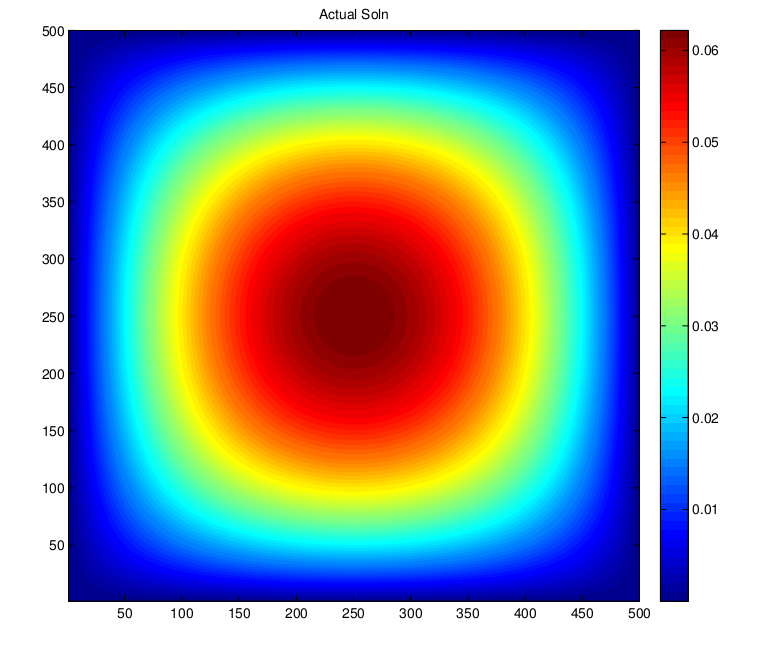
\includegraphics[height=0.4\textwidth, trim=0.2cm 0.2cm 0.2cm .2cm,clip=true]{figs/Poisson2D.png}}%
     %% 
	\:
	\subfigure[3D case on N$^3$ $= 100^3$]
   {\label{fig:Poisson 3D}	   
   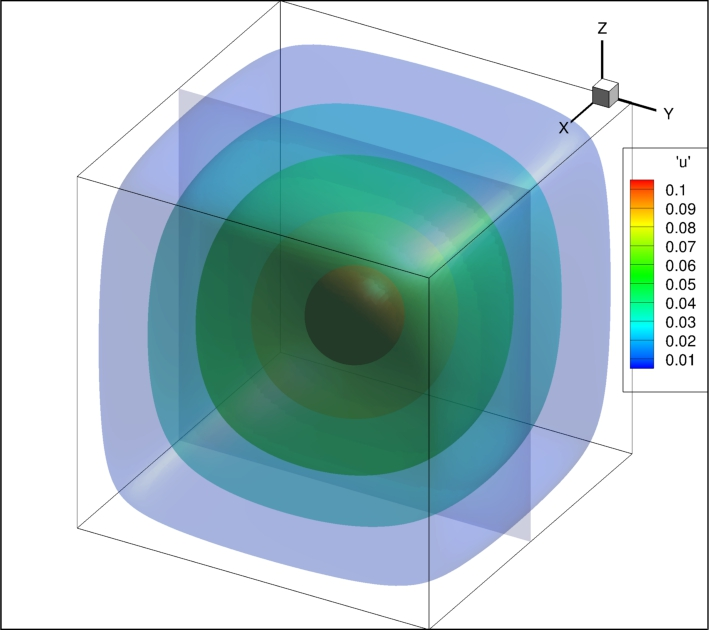
\includegraphics[height=0.4\textwidth, trim=0.2cm 0.2cm 0.2cm .2cm,clip=true]{figs/Poisson3D.jpeg}}%
     %%\caption{Solution Contours for the 3D solution of the Poisson Problem}  
     
    \caption{Solution Contours for solution of the Poisson Problem}  
\end{figure}

%%%%%%%%%%%%%%%%%%%%%%%%%%%%%%%%%%%%%%%%%%%%%%%%%%%%%%%%%%%%%%%%%%%%%%%%%%%%%%%%%%%%%%%%%%%%
%-------------------------------------------------------------------------------------------
% LES of Premixed Flames
%-------------------------------------------------------------------------------------------
%%%%%%%%%%%%%%%%%%%%%%%%%%%%%%%%%%%%%%%%%%%%%%%%%%%%%%%%%%%%%%%%%%%%%%%%%%%%%%%%%%%%%%%%%%%%
\section{LES of a Turbulent Premixed Methane Flame}
\subsection{Model Problem}


\begin{figure}
    \vspace{0.2cm}
    \begin{center}
      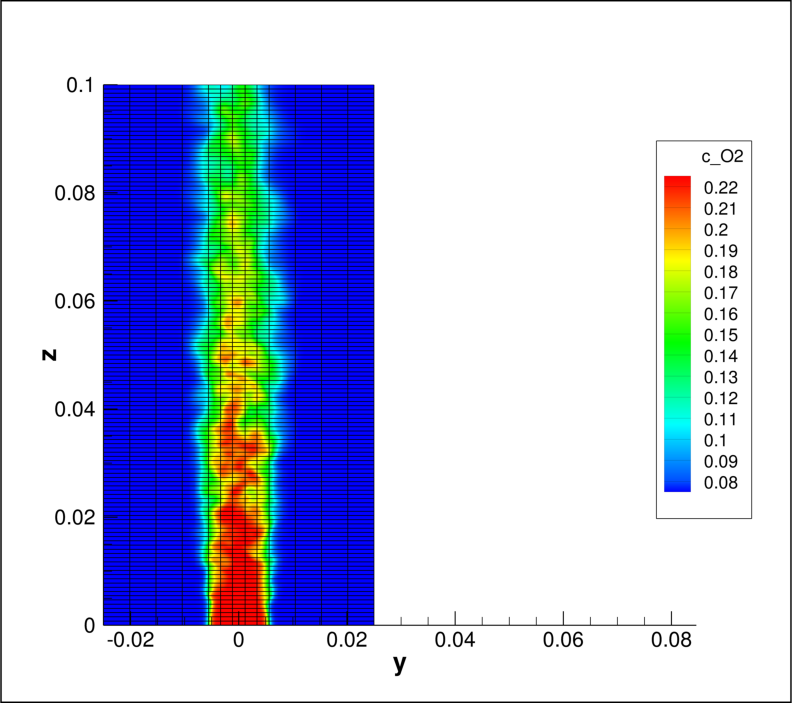
\includegraphics[height=0.4\textwidth]{./figs/Time_averaged_c_O2.png}
    \end{center}
    \caption{Time averaged $O_2$ species concentration}  
    \vspace{0.2cm}
    \label{fig:oxygen}	
\end{figure}

The CFFC code was used to run a simulation for a Turbulent Premixed Methane flame, using 800 nodes, 3200 blocks and each block having $8^3 = 512$ cells, hence a total of $1,638,400$ cells. Time averaged results for t=6ms, 7ms, 8ms, 9ms, 10ms and 11ms are shown in figure \ref{fig:oxygen}, the contours representing the species concentration of Oxygen.\par


Included here are some pictures from previous CFFC simulations that show the varying mesh cell sizes among the different blocks.

\begin{figure}[t!]
  \centering
   \subfigure[At t=2.0ms, 800 (8x8x8) blocks, ~410,000 cells
(no refinement, 1 mesh level)]
   {\label{fig:2msflame}	   
   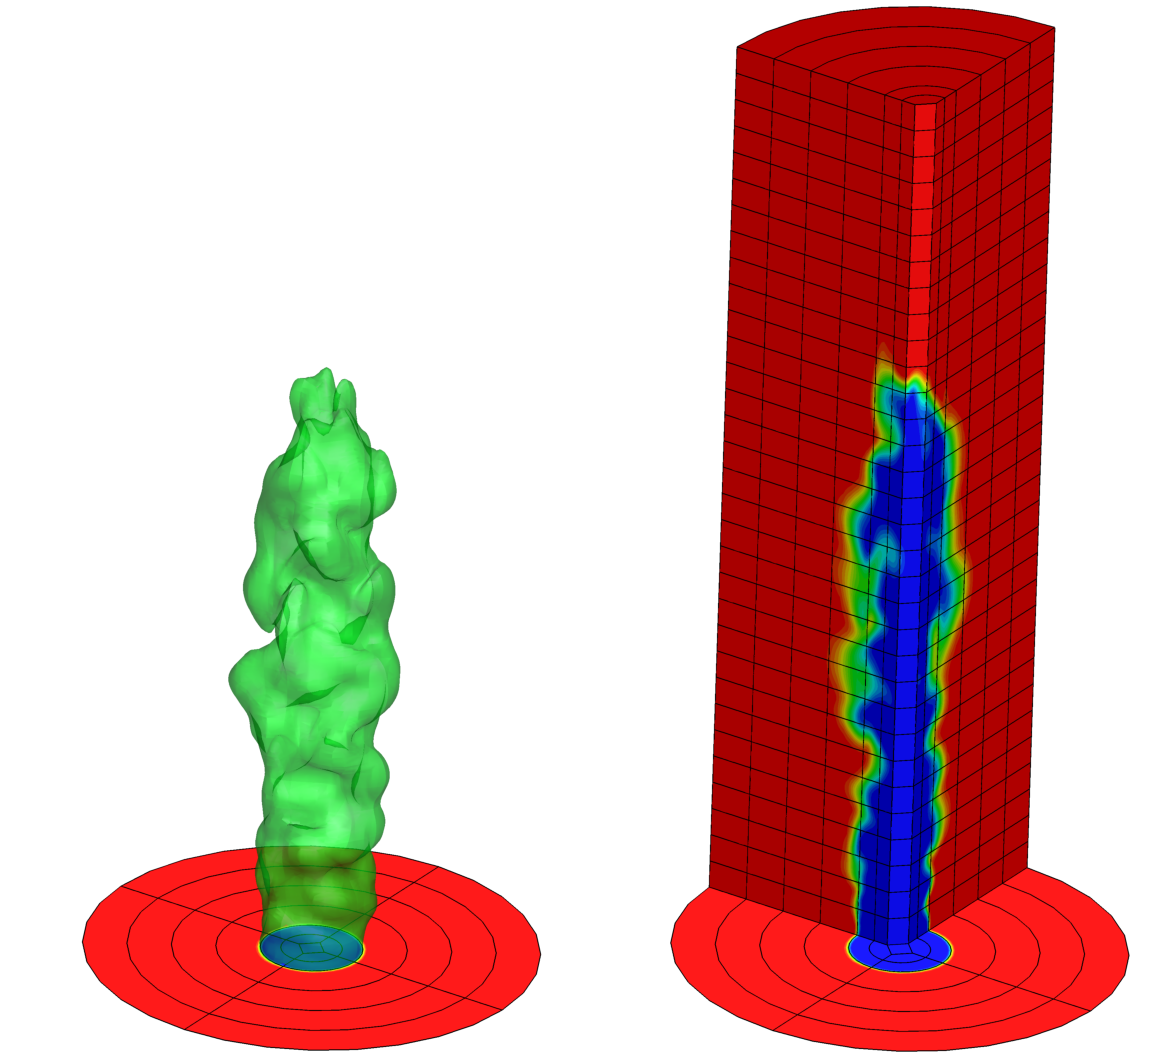
\includegraphics[height=0.25\textwidth]{figs/fsd2_0ms.png}}%
	\:
	\subfigure[At t=4.25ms 5595 (8x8x8) blocks, ~2.8 million cells
(3 levels of mesh refinement)]
   {\label{fig:4msflame}	   
   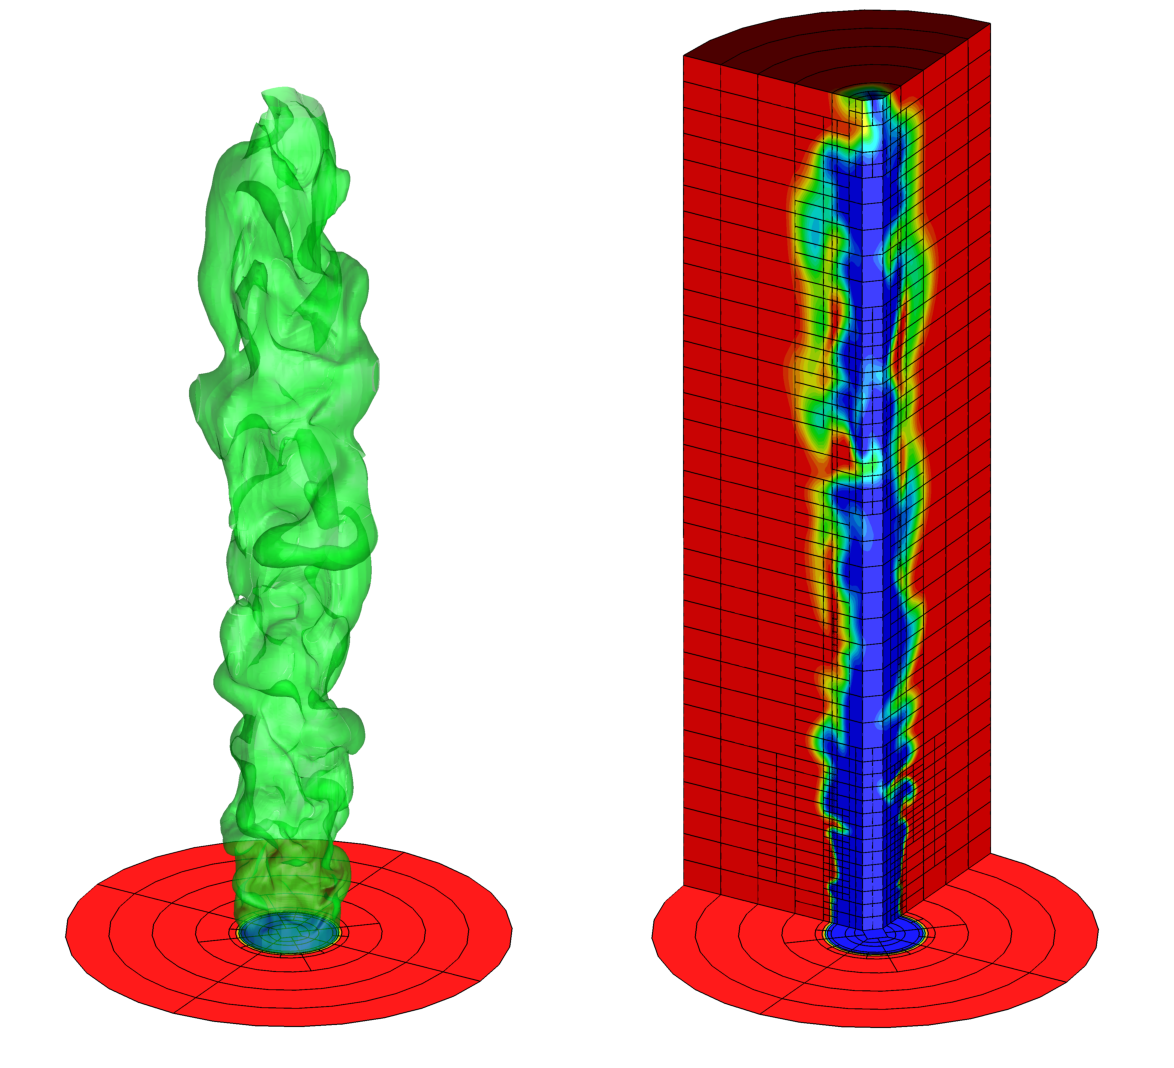
\includegraphics[height=0.25\textwidth]{figs/fsd4_25ms.png}}%
   \:
	\subfigure[At 7.0 ms, 18531 (8x8x8) blocks, ~9.5 million cells
(3 levels of mesh refinement)]
   {\label{fig:7msflame}	   
   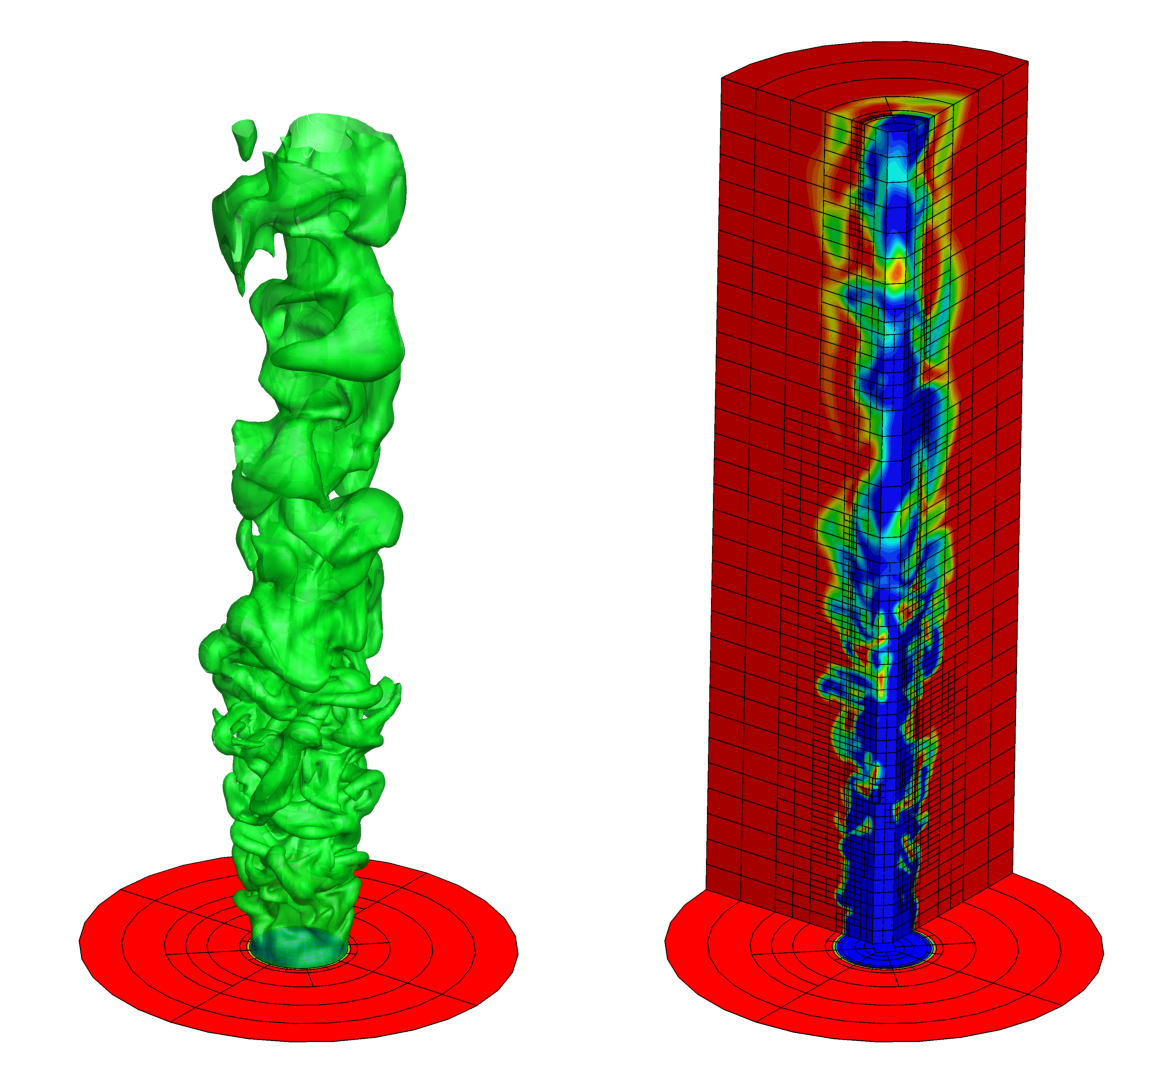
\includegraphics[height=0.25\textwidth]{figs/fsd7_0ms.png}}%
   \caption{Some figures showing isotropic mesh refinement with 3 levels of refinement for a lean premixed methane air flame in air. LES solutions were obtained with the flame surface density (FSD) model and the refinement was based on temperature gradient.} 
      
\end{figure}  




%%%%%%%%%%%%%%%%%%%%%%%%%%%%%%%%%%%%%%%%%%%%%%%%%%%%%%%%%%%%%%%%%%%%%%%%%%%%%%%%%%%%%%%%%%%%
%-------------------------------------------------------------------------------------------
% Adjoint Cases run
%-------------------------------------------------------------------------------------------
%%%%%%%%%%%%%%%%%%%%%%%%%%%%%%%%%%%%%%%%%%%%%%%%%%%%%%%%%%%%%%%%%%%%%%%%%%%%%%%%%%%%%%%%%%%%
\subsection{Discrete adjoint solutions on a shock cube problem}
\label{subsection:Discrete_Adjoint}

Following the adjoint formulation explained in Section \ref{section:Adjoint} it is seen that the adjoint formulation (also known as the \textit{dual problem}) can be written as a linear system:

\begin{equation}
\mathbf{A}^T\mathbf{x} = -\mathbf{b}^T
\end{equation}

Thus we can write the transpose of the residual Jacobian matrix, ${\partial{R}}/{\partial{U}}$ as matrix $A^T$ and the right hand side vector $\mathbf{b}$ as the derivative of the functional with respect to the state, ${\partial{J}}/{\partial{\mathbf{U_i}}}$\par

Adjoint sensitivities were evaluated for a shock cube problem governed by the Euler equations (see figure \ref{fig:Adjoints}). The initial conditions were ${\rho_R}/{\rho_L} = 8$, ${P_R}/{P_L} = 10$. Average pressure in the entire domain was selected as the functional, $J$. \par

\begin{figure}[t!]
  \centering
   \subfigure[Initial conditions for density showing large jump between left and right states]
   {\label{fig:init_cond}	   
   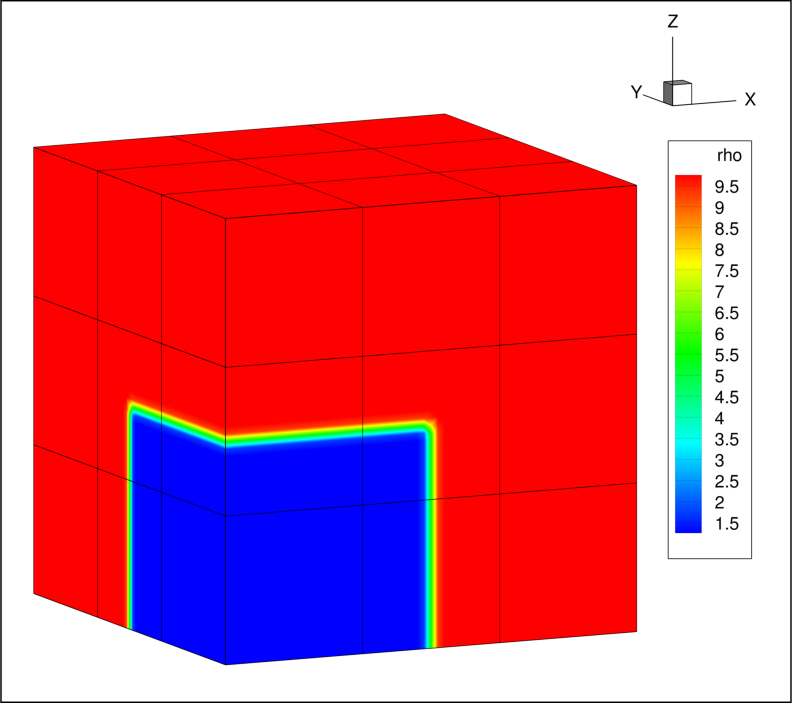
\includegraphics[height=0.45\textwidth]{figs/20Rho.png}}%
   \subfigure[sensitivity to Density]
   {\label{fig:rho_Adjoint}	   
   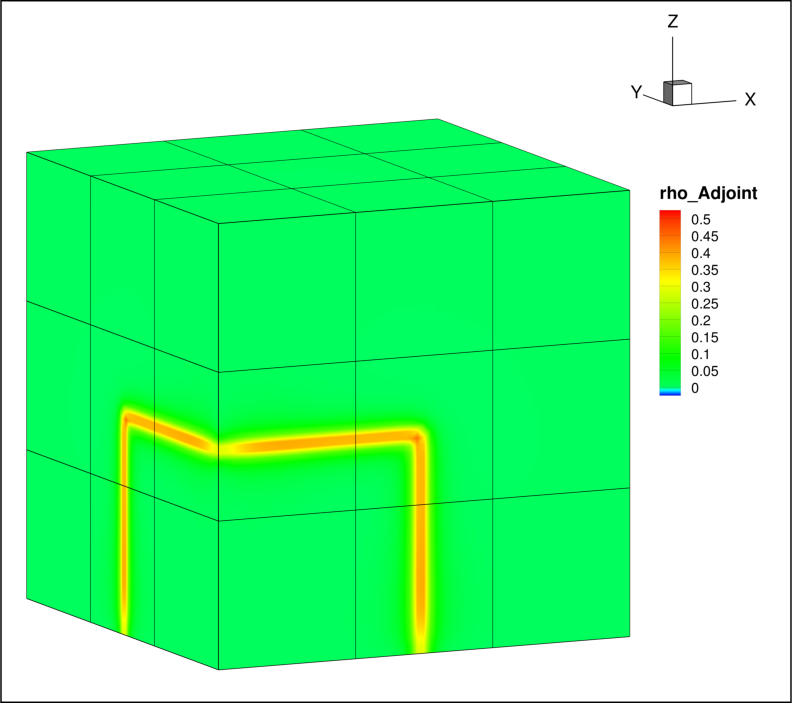
\includegraphics[height=0.45\textwidth]{./figs/20RhoAdj.png}}%
\caption{Contours of $\rho$ and adjoint $\psi_{\rho}$ at t = 0 sec. 27 (20x20x20) blocks} 
\label{fig:Adjoints}      
\end{figure}  



%%%%%%%%%%%%%%%%%%%%%%%%%%%%%%%%%%%%%%%%%%%%%%%%%%%%%%%%%%%%%%%%%%%%%%%%%%%%%%%%%%%%%%%%%%%%
%-------------------------------------------------------------------------------------------
% Summary of Progress to Date and Future Work
%-------------------------------------------------------------------------------------------
%%%%%%%%%%%%%%%%%%%%%%%%%%%%%%%%%%%%%%%%%%%%%%%%%%%%%%%%%%%%%%%%%%%%%%%%%%%%%%%%%%%%%%%%%%%%
\newpage
\section{Summary of progress to date and future work}

\subsection{Progress to date}

\begin{tabular}{|l|c|} \hline
\multicolumn{1}{|c|}{\bf{Task}} & \multicolumn{1}{|c|}{\bf{Completion Date}} \\

\hline Literature Review & September-October 2014 \\

\hline Trelis Meshing Software & November 2014 \\

\hline CFFC Group Code Flux Jacobian Analysis & December 2014 \\

\hline Trilinos Package solution for example Poisson Problem & December 2014 \\in serial and parallel configurations & \\

\hline Running a current-state LES case of a Turbulent Premixed & January 2015 \\Methane Flame using PCM-FPI to get a threshold estimation & \\ of solution run time &\\

\hline Implementing the approximate Adjoint Derivative to the Flux Jacobians & March 2015 \\ testing on Euler Equations  &\\

\hline
\end{tabular}

\subsection{Future work}

\begin{tabular}{|l|c|} \hline
\multicolumn{1}{|c|}{\bf{Task}} & \multicolumn{1}{|c|}{\bf{Completion Date}} \\

\hline Extension to Mesh adaptation & May 2015\\

\hline Application of Adjoint Problem to Navier Stokes  & June 2015\\

\hline Explicit Filters for High Order FVM implementation  & October 2015\\

\hline Conference Paper I draft & November 2015\\

\hline Coupling of High Order method with Adjoint-based AMR & December 2015\\

\hline CFD simulation of Cold Flow & January 2016\\

\hline CFD simulation of Laminar Non-Premixed Flame & February 2016\\

\hline CFD simulation of Laminar Premixed Flame & June 2016\\

\hline Journal Paper I & April 2016\\

\hline Conference Paper II draft & April 2016\\

\hline Journal Paper II & July 2016\\

\hline Conference Paper I Presentation  & July 2016\\

\hline Conference Paper II draft  & October 2016\\

\hline CFD simulation of Turbulent Non-Premixed Flame & October 2016\\

\hline Journal Paper III & October 2016\\

\hline Conference Paper III draft  & November 2016\\

\hline CFD simulation of Turbulent Non-Premixed Flame & March 2017\\

\hline Thesis write-up & September 2017 \\ 

\hline

\end{tabular}


\newpage
%%=================================================
\section{Appendix} 
\setcounter{equation}{0}
\subsection{Navier Stokes Equations} \label{section:Navier}
The conservation equations
for a thermally perfect reactive mixture of $N$ chemical species
evolving in time, $t$, and space, $\Vector{x}$, can then be written
using tensor notation as \cite{HPerez:2011}\par
%
\indent Conservation of Mass:
\begin{equation}
  \label{eq:mass}
  \frac{\partial \rho}{\partial t} 
  + \frac{\partial (\rho u_j)}{\partial x_j}  =  0 \,,
\end{equation}
%
\indent Conservation of Momentum:
\begin{equation}
  \label{eq:momentum} 
  \frac{\partial (\rho u_i)}{\partial t} 
  + \frac{\partial (\rho u_i u_j + \delta_{ij} p)}{\partial x_j}  
  - \frac{\partial \tau_{ij}}{\partial x_j}
  =  \rho g_i \,, 
\end{equation}
%
\indent Conservation of Energy:
\begin{equation}
  \label{eq:energy}
  \frac{\partial (\rho E)}{\partial t} 
  + \frac{\partial [(\rho E + p) u_j]}{\partial x_j} 
  - \frac{\partial (\tau_{ij} u_i)}{\partial x_j} 
  + \frac{\partial q_j}{\partial x_j}
  =  \rho g_i u_i \,,  
\end{equation}
%
\indent Conservation of Species Fraction:
\begin{equation}
  \label{eq:species}
  \frac{\partial (\rho Y_\alpha)}{\partial t} 
  + \frac{\partial (\rho Y_\alpha u_j)}{\partial x_j}
  + \frac{\partial \mathcal{J}_{j,\alpha} }{\partial{x_j}} 
  =  \dot{\omega}_{\alpha} \,, 
\end{equation}
%
where
%
\begin{eqnarray}
  \label{eq:stress_tensor}
  \tau_{ij} & = & \mu \left( \frac{\partial u_i}{\partial x_j} 
  + \frac{\partial u_j}{\partial x_i} \right) 
  - \frac{2}{3} \mu \delta_{ij} \frac{\partial u_l}{\partial x_l} \,,  \\
  \label{eq:heat_flux}
  q_j & = & - \lambda \frac{\partial T}{\partial x_j} 
  - \rho \sum_{\alpha=1}^N h_\alpha\mathcal{D}_\alpha \frac{\partial Y_\alpha}{\partial x_j}  \,, \\
  \label{eq:species_diffusive_flux}
  \mathcal{J}_{j,\alpha} & = & - \rho \mathcal{D}_\alpha \frac{\partial Y_\alpha}{\partial x_j} \,,  
\end{eqnarray}
%



%%===================================================
\subsection{Favre-Averaged Navier Stokes Equations} \label{section:Favre}
Favre-Filtering, essentially a density-weighted filtering procedure is defined as:
\begin{equation}
 \tilde{\phi}=\frac{\overline{\rho \phi}}{\overline{\rho}},
 \end{equation}
where $\tilde{\phi}$ represents the Favre-filtered variable.

Performing this on the governing equations, and assuming that the differentiation and filtering operations commute, we obtain the Favre-Filtered Equations \cite{HPerez:2011}:\par

Conservation of Mass:
\begin{equation}
  \label{eq:filt_mass} 
  \Pfrac{\bar{\rho}}{t} + \Pfrac{(\bar{\rho} \tilde{u}_j )}{x_j} = 0 \,,
\end{equation}
%
\indent Conservation of Momentum:
\begin{equation} 
  \label{eq:filt_momentum}
  \Pfrac{( \bar{\rho} \tilde{u}_i )}{t} 
  + \Pfrac{( \bar{\rho} \tilde{u}_i \tilde{u}_j + \delta_{ij} \bar{p} )}{x_j} 
  - \Pfrac{\check{\tau}_{ij}}{x_j} 
  =  \bar{\rho} g_i 
  + \underbrace{\Pfrac{\sigma_{ij}}{x_j}}_{\bf I}
  + \underbrace{\Pfrac{( \bar{\tau}_{ij} - \check{\tau}_{ij} )}{x_j}}_{\bf II} \,,
\end{equation}
%
\indent Conservation of Energy:
\begin{eqnarray}
  \label{eq:filt_energy}
  \Pfrac{( \bar{\rho} \tilde{E} )}{t} 
  + \Pfrac{[ (\bar{\rho} \tilde{E} + \bar{p}) \tilde{u}_j ]}{x_j}  
  - \Pfrac{( \check{\tau}_{ij} \tilde{u}_i )}{x_j}  
  + \Pfrac{\check{q}_j}{x_j} 
  & = & 
  \bar{\rho} \tilde{u}_i g_i
  - \underbrace{\Pfrac{[ \bar{\rho} (\widetilde{h_{\mathrm{s}} u_j} - \check{h}_{\mathrm{s}} \tilde{u}_j) ]}{x_j}
  }_{\bf III} 
  {} \nonumber \\  &  & {} 
  \!\!\!\!\! + \underbrace{\Pfrac{(\overline{\tau_{ij} u_i} - \check{\tau}_{ij} \tilde{u}_i)}{x_j}
  }_{\bf IV}
  - \underbrace{\Pfrac{(\bar{q}_j - \check{q}_j)}{x_j}}_{\bf V}
  {} \nonumber \\   &  & {} 
  \!\!\!\!\! - \underbrace{ \frac{1}{2} \Pfrac{[ \bar{\rho} (\widetilde{u_j u_i u_i}
      - \tilde{u}_j \widetilde{u_i u_i}) ]}{x_j}}_{\bf VI}
  {} \nonumber \\  &  & {}
  \!\!\!\!\! - \underbrace{\Pfrac{[ \sum_{\alpha=1}^N \Delta h^0_{\mathrm{f}_\alpha} \bar{\rho}
      (\widetilde{Y_\alpha u_{j}} - \tilde{Y}_\alpha \tilde{u}_j) ]}{x_j} \,,
  }_{\bf VII}
\end{eqnarray}
%
\indent Conservation of Species Fraction:
\begin{equation} 
  \label{eq:filt_species}
  \Pfrac{( \bar{\rho} \tilde{Y}_\alpha )}{t} 
  + \Pfrac{( \bar{\rho} \tilde{Y}_\alpha \tilde{u}_j )}{x_j}
  + \Pfrac{\check{\cal J}_{j,\alpha}}{x_j} 
  = - \underbrace{\Pfrac{[ \bar{\rho}(\widetilde{Y_\alpha u_j} - 
                  \tilde{Y}_\alpha \tilde{u}_j) ]}{x_j}}_{\bf VIII} 
  - \underbrace{\Pfrac{(\bar{\cal J}_{j,\alpha} - \check{\cal J}_{j,\alpha})}{x_j}}_{\bf IX} 
  + \underbrace{\bar{\dot{\omega}}_\alpha}_{\bf X} \,,
\end{equation}
%
Where we use the equation of state:
\begin{equation} 
  \label{eq:filt_eq_state} 
  \bar{p} = \bar{\rho} \check{R} \tilde{T} 
  + \underbrace{ \sum_{\alpha=1}^N R_\alpha \bar{\rho}
    (\widetilde{Y_\alpha T} - \tilde{Y}_\alpha \tilde{T}) }_{\bf XI} \,,
\end{equation}
%
%
where
%
\begin{equation}
  \label{eq:sfs_stresses}
  \sigma_{ij} = - \bar{\rho} \left( \widetilde{u_i u_j} - \tilde{u}_i \tilde{u}_j \right) \,, 
\end{equation}
%                     
is the SFS stress tensor. The total energy is written as:
%
\begin{equation}
  \tilde{E} = \check{h}_{\mathrm{s}} - \frac{\bar{p}}{\bar{\rho}} 
  + \sum_{\alpha=1}^N \Delta h^0_{\mathrm{f}_\alpha} \tilde{Y}_\alpha 
  + \frac{1}{2}\tilde{u}_i \tilde{u}_i + k_\Delta \,,
\end{equation}
%
where
% 
\begin{equation}
  k_\Delta = \frac{1}{2} \left( \widetilde{u_i u_i} - \tilde{u_i}\tilde{u_i} \right) \,,
\end{equation}
%
is the Sub-Filter Scale (SFS) Turbulent Kinetic Energy. The effects of the subfilter scales appear in the filtered total energy, $\tilde{E}$, the filtered
equation of state and the right-hand-sides of the governing continuity, momentum, energy and species mass fraction equations (i.e., terms \textbf{I},\ldots,\textbf{XI}). The symbol $(\,\check{}\,)$ is used to indicate the evaluation of expressions in terms of filtered variables, i.e.,
$\check{R}\!=\!R(\tilde{Y}_\alpha)$,
$\check{h}_{\mathrm{s}}\!=\!h_{\mathrm{s}}(\tilde{Y}_\alpha,\tilde{T})$,
and so on. The fluxes $\check{\tau}_{ij}$, $\check{q}_j$, and
$\check{\cal J}_{j,\alpha}$ are expressed as
%
\begin{eqnarray}
  \check{\tau}_{ij} & = &  2 \check{\mu} \left( \check{S}_{ij} - 
  \frac{1}{3} \delta_{ij}\check{S}_{ll} \right) \,,  \\
%
  \check{q}_j & = &  - \check{\lambda} \frac{\partial \tilde{T}}{\partial x_j} 
  - \bar{\rho} \sum_{\alpha=1}^N \check{h}_\alpha \check{D}_\alpha \frac{\partial \tilde{Y}_\alpha}{\partial x_j} \,, \\
%
  \check{\cal J}_{j,\alpha} & = &  - \bar{\rho} \check{D}_\alpha \frac{\partial \tilde{Y}_\alpha}{\partial x_j} \,,
\end{eqnarray}
%
where 
%
$\check{S}_{ij} \!=\! \frac{1}{2} \left(\partial \tilde{u}_{i}/\partial
  x_{j} + \partial \tilde{u}_j/ \partial x_i \right)$, is the strain rate tensor calculated with the Favre-filtered velocity.  The temperature used for the molecular transport coefficients $\check{\mu}$, $\check{\lambda}$, and $\check{D}_\alpha$ calculations is $\tilde{T}$.

Modelling of the SFS terms is required to close the above system of equations. Term \textbf{II} is neglected under the assumption that the filtered viscous stresses, $\bar{\tau}_{ij}$, can be approximated to the viscous stresses evaluated in terms of the Favre-filtered velocity, $\check{\tau}_{ij}$. Following similar assumptions for the total heat and species mass diffusion fluxes, terms \textbf{V} and
\textbf{IX} may be neglected. Vreman \etal ~\cite{vreman:1995} performed a priori LES of a mixing layer at different Mach numbers and concluded that neglecting the non-linearities of the diffusion terms in the momentum and energy equations is acceptable. Regarding term \textbf{IV} (SFS viscous diffusion), it is generally much smaller than the other terms that require a model~\cite{martin:2000}, and so is neglected. As for term \textbf{XI} (SFS temperature-species correlation), it is assumed to be small and generally neglected.
%
Following the work of Knight \etal.~\cite{knight:1998}, term \textbf{VI} (the SFS turbulent diffusion) can be modelled in terms of the SFS stresses and the resolved velocity as
%
\begin{equation}
  - \frac{\bar{\rho} \left(\widetilde{u_j u_i u_i} - \tilde{u}_j\widetilde{u_i u_i} \right)}{2} 
  = \sigma_{ij}\tilde{u}_i \,.
\end{equation}
%
Term \textbf{VII} involves the SFS species fluxes (term \textbf{VIII}) and is closed with the modelled SFS species fluxes. 
%\newpage
%%\bibliographystyle{aiaa}
\bibliography{journals-full,cfd,chris_ref}
\end{document}
